\documentclass[11pt,a4paper]{article}
\usepackage[margin=24mm,headheight=14pt]{geometry}
\usepackage[T1]{fontenc}
\usepackage{lmodern}
\usepackage{microtype}
\usepackage{xcolor}
\usepackage{graphicx}
\usepackage{booktabs}
\usepackage{tabularx}
\usepackage{array}
\usepackage{longtable}
\usepackage{enumitem}
\usepackage{tikz}
\usetikzlibrary{arrows.meta,positioning,fit,shapes.geometric}
\usepackage{fancyhdr}
\usepackage[hidelinks]{hyperref}
\usepackage{titlesec}

\definecolor{ehgreen}{HTML}{245B43}
\definecolor{ehmint}{HTML}{EAF2ED}
\definecolor{ehgray}{HTML}{56625B}
\definecolor{ehline}{HTML}{D9E1DB}
\hypersetup{colorlinks=true,linkcolor=ehgreen,urlcolor=ehgreen,citecolor=ehgreen}
\pagestyle{fancy}
\fancyhf{}
\lhead{\small EasyHousing | High-Level Design}
\rhead{\small Version 1.0}
\cfoot{\thepage}
\setlength{\parskip}{5pt}
\setlength{\parindent}{0pt}
\setlist[itemize]{leftmargin=18pt,itemsep=2pt,topsep=3pt}
\setlist[enumerate]{leftmargin=20pt,itemsep=2pt,topsep=3pt}
\titleformat{\section}{\Large\bfseries\color{ehgreen}}{\thesection}{0.7em}{}
\titleformat{\subsection}{\large\bfseries\color{ehgray}}{\thesubsection}{0.7em}{}
\newcommand{\code}[1]{\texttt{\detokenize{#1}}}
\newcommand{\service}[1]{\textbf{#1}}
\newcommand{\tagline}[1]{{\large\color{ehgray}#1}}

\begin{document}
\begin{titlepage}
\centering
\vspace*{25mm}
{\color{ehgreen}\rule{\textwidth}{2pt}}\par
\vspace{14mm}
{\Huge\bfseries EasyHousing\par}
\vspace{5mm}
{\LARGE High-Level Design\par}
\vspace{6mm}
\tagline{System architecture, service boundaries, and quality attributes}\par
\vspace{15mm}
{\color{ehgreen}\rule{0.62\textwidth}{1pt}}\par
\vspace{19mm}
\begin{tabular}{rl}
\textbf{Document type:} & High-Level Design (HLD)\\
\textbf{System:} & EasyHousing property discovery and listing platform\\
\textbf{Implementation:} & Angular 22, ASP.NET Core/.NET 8, SQL Server\\
\textbf{Revision:} & 1.0\\
\textbf{Prepared:} & November 2026\\
\textbf{Source baseline:} & Current EasyHousingSolution workspace\\
\end{tabular}
\vfill
\begin{minipage}{0.82\textwidth}
\small\color{ehgray}
This document describes the architecture found in the repository. It distinguishes
implemented behavior from future operational recommendations; it is not a claim that
unimplemented production infrastructure is already deployed.
\end{minipage}
\vspace{12mm}
\end{titlepage}

\tableofcontents
\newpage

\section{Document Purpose and System Context}
EasyHousing is a web application for property discovery and listing management. Buyers
can search verified listings, inspect details, compare homes, reveal owner contact
information, and save properties. Sellers can create and edit listings and upload
photos. Administrators review, verify, and deactivate properties.

This HLD gives product and engineering stakeholders a shared view of the current
system boundaries, runtime topology, trust boundaries, data ownership, and major
design decisions. The companion Low-Level Design describes service contracts and
implementation details.

\subsection{In scope}
\begin{itemize}
  \item The Angular single-page application with server-rendering support.
  \item The API gateway and Identity, User, Property, and Cart microservices.
  \item Service-owned relational databases and synchronous HTTP dependencies.
  \item Authentication, role authorization, property review, and image handling.
  \item Local development deployment and the principal quality constraints.
\end{itemize}

\subsection{Out of scope and important product boundary}
The current application records buyer-saved properties; it does not implement a
payment processor, escrow, title transfer, or a verified transaction workflow.
There is no message broker, distributed cache, object-storage service, or separately
deployed monitoring stack in the repository. Such capabilities must not be inferred
from the microservice layout.

\subsection{Stakeholders and principal actors}
\begin{tabularx}{\textwidth}{>{\bfseries}p{28mm} X}
\toprule
Actor & Primary goals and capabilities\\
\midrule
Visitor & Browse active, verified listings and view public property information.\\
Buyer & Register, authenticate, compare listings, reveal owner contact, manage saved homes.\\
Seller & Register with location details, submit/edit properties, upload property photos.\\
Administrator & Review submissions, verify listings, and deactivate active listings with a reason.\\
Operator/developer & Configure services and databases, run the local stack, inspect Swagger APIs.\\
\bottomrule
\end{tabularx}

\section{Architectural Drivers and Principles}
\subsection{Drivers}
\begin{enumerate}
  \item Separate identity, profile/location, property, and saved-home ownership.
  \item Keep a simple browser-facing API origin while routing requests to services.
  \item Enforce seller, buyer, and admin permissions at the API boundary, not only in the UI.
  \item Support property images and location-aware listings without a shared database.
  \item Keep local development reproducible with the .NET SDK and SQL Server LocalDB.
\end{enumerate}

\subsection{Design principles}
\begin{itemize}
  \item \textbf{Service data ownership:} Each business service writes only its own database.
  \item \textbf{HTTP integration:} Cross-service queries and commands use typed HTTP clients.
  \item \textbf{API-level trust:} JWT role checks protect business endpoints; internal
  profile operations use a shared internal API key.
  \item \textbf{Explicit lifecycle:} New properties enter \code{Pending}; verification
  activates them; an edit returns them to review.
  \item \textbf{Documented reality:} The current gateway is a lightweight proxy, not a
  full API-management platform, and LocalDB is a development database choice.
\end{itemize}

\section{System Context and Runtime Topology}
The browser uses the Angular app on port 4200 and sends API calls to the gateway on
port 5200. The gateway forwards a request to one downstream service based on the
first API path segment. Services are independently hosted ASP.NET Core applications.

\begin{figure}[h!]
\centering
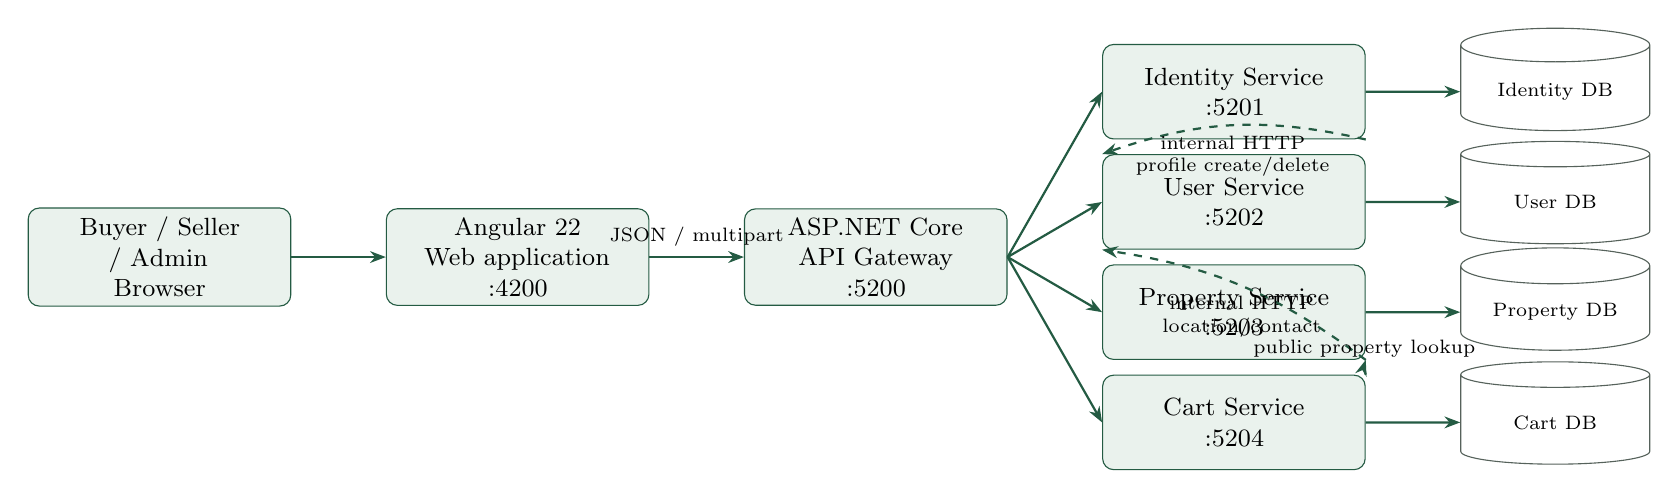
\begin{tikzpicture}[
  node distance=9mm and 12mm,
  box/.style={draw=ehgreen,fill=ehmint,rounded corners,align=center,
    minimum width=31mm,minimum height=12mm,text width=31mm,font=\small},
  db/.style={draw=ehgray,fill=white,cylinder,shape border rotate=90,
    aspect=0.25,minimum width=24mm,minimum height=13mm,align=center,font=\scriptsize},
  edge/.style={-{Stealth[length=2mm]},thick,draw=ehgreen}
]
\node[box] (browser) {Buyer / Seller / Admin\\Browser};
\node[box,right=of browser] (web) {Angular 22\\Web application\\:4200};
\node[box,right=of web] (gateway) {ASP.NET Core\\API Gateway\\:5200};
\node[box,right=of gateway,yshift=21mm] (identity) {Identity Service\\:5201};
\node[box,right=of gateway,yshift=7mm] (user) {User Service\\:5202};
\node[box,right=of gateway,yshift=-7mm] (property) {Property Service\\:5203};
\node[box,right=of gateway,yshift=-21mm] (cart) {Cart Service\\:5204};
\node[db,right=of identity] (idb) {Identity DB};
\node[db,right=of user] (udb) {User DB};
\node[db,right=of property] (pdb) {Property DB};
\node[db,right=of cart] (cdb) {Cart DB};
\draw[edge] (browser) -- (web);
\draw[edge] (web) -- node[above,font=\scriptsize]{JSON / multipart} (gateway);
\draw[edge] (gateway.east) -- (identity.west);
\draw[edge] (gateway.east) -- (user.west);
\draw[edge] (gateway.east) -- (property.west);
\draw[edge] (gateway.east) -- (cart.west);
\draw[edge] (identity) -- (idb);
\draw[edge] (user) -- (udb);
\draw[edge] (property) -- (pdb);
\draw[edge] (cart) -- (cdb);
\draw[edge,dashed] (identity.south east) to[bend right=16]
  node[below,font=\scriptsize,align=center]{internal HTTP\\profile create/delete} (user.north west);
\draw[edge,dashed] (property.south east) to[bend right=14]
  node[below,font=\scriptsize,align=center]{internal HTTP\\location/contact} (user.south west);
\draw[edge,dashed] (cart.north east) to[bend left=18]
  node[above,font=\scriptsize,align=center]{public property lookup} (property.south east);
\end{tikzpicture}
\caption{Logical application topology. Dashed arrows denote service-to-service HTTP calls.}
\end{figure}

\subsection{Local endpoints}
\begin{tabularx}{\textwidth}{>{\bfseries}p{31mm} p{26mm} X}
\toprule
Component & HTTP port & Responsibility\\
\midrule
Angular frontend & 4200 & Browser UI; configured API origin is \code{http://localhost:5200/api}.\\
API Gateway & 5200 & Path-based HTTP proxy; aggregates development Swagger documents.\\
Identity Service & 5201 & Login, registration, password hashing, JWT issuance.\\
User Service & 5202 & Profiles, state/city catalog, internal contact/location operations.\\
Property Service & 5203 & Listing lifecycle, image upload and property queries.\\
Cart Service & 5204 & Buyer-specific saved-property persistence and property lookup.\\
\bottomrule
\end{tabularx}

\section{Service Boundaries and Responsibilities}
\begin{longtable}{>{\bfseries}p{27mm} p{43mm} p{44mm} p{30mm}}
\toprule
Service & Owns & Exposes (summary) & Depends on\\
\midrule
\endhead
API Gateway & Routing configuration only; no business database & \code{/api/identity/*},
\code{/api/locations/*}, \code{/api/properties/*}, \code{/api/cart/*}; development Swagger proxy
& Identity, User, Property, Cart\\
Identity & Account username, password hash, role, profile identifier & Register and login;
issues signed eight-hour JWTs & User Service for profile creation and compensation\\
User & Buyer/seller contact profile and state/city catalogue & Public location reads;
internal-key protected profile, contact and region operations & None\\
Property & Listing status/data and image bytes/content type & Public search/details;
role-protected seller/admin operations; buyer contact lookup & User Service\\
Cart & Buyer/property saved-item records & Buyer-only list/add/remove & Property Service\\
\bottomrule
\end{longtable}

\subsection{Why this split}
Identity data is separated from personally identifiable profile data. The property
service owns listing data and its photos, so verification and image lifecycle remain
with the listing. The cart stores references rather than duplicating listing
snapshots; when the cart is read, it resolves current property details over HTTP.
Location data belongs to the user/profile service and is resolved to a canonical
\code{City, State} region by the property service.

\section{Major Business Flows}
\subsection{Registration and authentication}
Registration is a synchronous, two-service operation. Identity validates the
requested buyer/seller role and basic request fields, asks User Service to create a
profile using the internal key, hashes the password, and persists the account.
If account persistence fails with a database update conflict, Identity asks User
Service to delete the newly-created profile as a compensating action. Login verifies
the password hash and issues a JWT carrying user name, role, and \code{profileId}.

\subsection{Property publishing and moderation}
A seller creates a property only after selecting a valid state and city. Property
Service asks User Service to resolve that pair and stores a normalized region.
New properties are \code{Pending} and are not returned by public search. The
administrator verifies a pending record to make it \code{Verified} and active.
Editing a seller-owned property resets it to pending and inactive until reviewed
again. Admin deactivation sets a reason and removes it from public results.

\subsection{Discovery, photos, and saved homes}
Search returns active verified listings with image records. Images are stored as
bytes and serialized as Base64 together with their MIME type in property DTOs. The
frontend converts these values to data URLs for actual image elements. A buyer's
cart persists a property ID; the Cart Service resolves its current data from
Property Service when listing or validating saved items.

\section{Data Architecture}
There are four service-owned SQL Server databases:
\begin{itemize}
  \item \textbf{EasyHousingIdentity:} unique username, password hash, role, and user ID.
  \item \textbf{EasyHousingUser:} profiles, states, and cities; state/city foreign keys
  are restrictive and city is linked to its state.
  \item \textbf{EasyHousingProperty:} property listings and child image rows; deleting
  a listing cascades to its image rows.
  \item \textbf{EasyHousingCart:} saved property ID, buyer ID, and timestamp; a unique
  buyer/property index prevents duplicate saves.
\end{itemize}
The account-to-profile, property-to-seller, and cart-to-property links are identifiers
across service boundaries rather than cross-database foreign keys. Referential checks
for those links are performed by service logic or HTTP requests.

\subsection{Persistence and migration note}
The current service startup code uses Entity Framework Core
\code{EnsureCreatedAsync()} and seed logic for the location catalog and default admin.
This is suitable for the current local development baseline but is not a replacement
for a versioned production migration strategy. Schema changes must be planned
carefully before adopting migrations against existing LocalDB data.

\section{Security and Trust Boundaries}
\begin{itemize}
  \item The public browser boundary is the gateway. The current gateway forwards
  request headers, including Authorization, and does not itself enforce roles.
  Services validate JWT signature, issuer, audience, expiry, and role authorization.
  \item Protected operations require role claims: Seller for create/update/upload,
  Buyer for cart and owner contact/compare, Admin for moderation.
  \item Identity and User Service share development JWT issuer/audience/signing
  configuration. User Service uses an internal API key for profile and contact
  endpoints; it is a shared-secret boundary, not mutual TLS.
  \item Passwords are stored as hashes through ASP.NET Core's
  \code{PasswordHasher<T>}; plaintext passwords are not stored.
  \item Checked-in local configuration contains development keys and LocalDB
  connection strings. Production secrets must be injected through a protected
  configuration system, not copied from repository defaults.
  \item The browser stores session/token values in local storage. This architecture
  therefore requires XSS prevention and a security review before production use.
\end{itemize}

\section{Quality Attributes and Constraints}
\begin{tabularx}{\textwidth}{>{\bfseries}p{31mm} X}
\toprule
Attribute & Current design and implications\\
\midrule
Availability & Synchronous downstream calls mean a dependency outage can fail
registration, owner-contact, or cart operations. The gateway does not currently
provide retries, circuit breakers, or health aggregation.\\
Performance & Search includes image bytes in DTO responses. Base64 adds payload
overhead; each property accepts up to six images of 5 MB each. Pagination,
thumbnail variants, and external object storage are not implemented.\\
Security & JWT role enforcement is implemented in services. Internal-key secrecy,
HTTPS termination, rate limiting, upload inspection, and browser storage hardening
remain deployment concerns.\\
Maintainability & Service directories isolate code and databases; cross-service
contracts currently use HTTP JSON and manually aligned DTOs rather than generated
shared contracts.\\
Scalability & Stateless APIs can be replicated behind a load balancer, but local
database, image-in-DB payloads, and shared configuration are not production
scalability mechanisms.\\
Usability & Role-specific Angular screens surface validation, loading, and errors;
seller image previews refresh after upload.\\
\bottomrule
\end{tabularx}

\section{Deployment View and Operations}
For local development, start each .NET project with its \code{http} launch profile;
profiles bind ports 5200--5204. SQL Server LocalDB is the configured storage engine.
Run the frontend from \code{frontend} using \code{npm start}. The UI allows origin
\code{http://localhost:4200}; backend services and gateway allow that configured
origin through CORS. Development Swagger UI is available at
\code{http://localhost:5200/swagger} and proxies each service's OpenAPI document.

Before a production deployment, provision independent database instances or
schemas, secrets, TLS, backups, health/readiness endpoints, structured request
correlation, central logs/metrics, a migration pipeline, and a gateway with
timeouts/limits. These are recommendations, not current implemented capabilities.

\section{Risks, Decisions, and Evolution}
\begin{tabularx}{\textwidth}{>{\bfseries}p{35mm} X}
\toprule
Topic & Architecture decision / follow-up\\
\midrule
Images in relational storage & Current choice preserves atomic ownership and simple local setup.
For larger catalogs, move originals and generated thumbnails to object storage and
return short metadata/URLs.\\
Cross-service consistency & Registration uses a compensating profile deletion after a
specific account persistence conflict. More general retries, idempotency, and an
outbox/workflow are future work if multi-step workflows expand.\\
Gateway behavior & A hand-built transparent proxy keeps the deployment small. Add
request limits, timeouts, path allowlists, correlation and resilience before
Internet exposure.\\
Schema evolution & Replace bootstrap-only \code{EnsureCreatedAsync()} with reviewed,
versioned database migrations and backups when long-lived environments are introduced.\\
API contracts & Add contract tests and/or generated clients if DTO drift between the
frontend and Cart/Property service becomes a recurring risk.\\
\bottomrule
\end{tabularx}

\section{Repository Map and Related Design}
\begin{itemize}
  \item Backend services: \code{backend/services/<ServiceName>/}; C\# source under
  each project's \code{src/}.
  \item Frontend: \code{frontend/src/app}; API origin and models under
  \code{core/}, role-specific user journeys under \code{features/}.
  \item Detailed endpoint, DTO, persistence, validation, and error behavior:
  see \href{backendd-lld.tex}{EasyHousing Low-Level Design}.
\end{itemize}

\vfill
\begin{center}\small\color{ehgray}End of High-Level Design\end{center}
\end{document}
